\documentclass[12pt, a4paper]{report} % 'report' or 'book' is suitable for project documentation.

\setlength{\textfloatsep}{5pt plus 2pt minus 2pt}

% Redefining chapter format
\makeatletter
\def\@makechapterhead#1{%
  \vspace*{50\p@}%
  {\parindent \z@ \raggedright \normalfont
    \ifnum \c@secnumdepth >\m@ne
      \huge\bfseries \@chapapp\space \thechapter
      \par\nobreak
      \vskip 20\p@
    \fi
    \interlinepenalty\@M
    \LARGE\bfseries #1\par\nobreak
    \vskip 40\p@
  }}
\makeatother

% Redefining section format
\makeatletter
\renewcommand\section{\@startsection {section}{1}{\z@}%
                                   {-3.5ex \@plus -1ex \@minus -.2ex}%
                                   {2.3ex \@plus.2ex}%
                                   {\large\bfseries}}
\makeatother

\makeatletter
\renewcommand\subsection{\@startsection {subsection}{2}{\z@}%
                                   {-3.25ex\@plus -1ex \@minus -.2ex}%
                                   {1.5ex \@plus .2ex}%
                                   {\normalsize\bfseries}}
\makeatother



%%%%%%%%%%%%%%%%%%%%%%%%%%%%%%%%%%%%%%%%%%%%%%%%%%%%%%%%%%%%%%%%%%%%%%%%%%%%%%%
% Package Imports
%\usepackage[utf8]{inputenc} % commented out as per your instruction
%\usepackage[T1]{fontenc} % commented out as per your instruction
\usepackage{graphicx}  % for including images
\usepackage{listings}  % for including code
\usepackage{hyperref}  % for hyperlinks
\usepackage{amsmath}   % for advanced math typesetting
\usepackage{geometry}  % for custom margins if needed
\usepackage{pdfpages}
\usepackage{longtable}
\usepackage{lscape}
%\usepackage{subfig}
\usepackage{makecell}
\usepackage{colortbl}
\usepackage{titlesec}
\usepackage{geometry}
\usepackage{subcaption}
\usepackage{adjustbox}
\usepackage{float}
\usepackage{placeins}
% to show directory trees
\usepackage{dirtree}
%\usepackage{forest}

\usepackage{pdfpages}

\usepackage{tikz}
\usetikzlibrary{trees}
\usepackage{listings}
\usepackage{xcolor}
\usepackage{caption}

\lstset{
  abovecaptionskip=10pt,
  belowcaptionskip=-6pt % Adjust this to your liking, negative values decrease the space
}

%\captionsetup[lstlisting]{belowskip=6pt} % Adjust 12pt to your liking
%\captionsetup[lstlisting]{aboveskip=6pt} % Adjust 12pt to your liking
\captionsetup[figure]{aboveskip=10pt} % Adjust 12pt to your liking


\lstdefinestyle{jsonstyle}{
    basicstyle=\ttfamily\small,
    numbers=left,
    numberstyle=\tiny,
    numbersep=8pt,
    breaklines=true,
    frame=tb,
    backgroundcolor=\color[RGB]{245,245,245},
    literate=
     *{0}{{{\color[RGB]{0,128,255}0}}}{1}
      {1}{{{\color[RGB]{0,128,255}1}}}{1}
      {2}{{{\color[RGB]{0,128,255}2}}}{1}
      {3}{{{\color[RGB]{0,128,255}3}}}{1}
      {4}{{{\color[RGB]{0,128,255}4}}}{1}
      {5}{{{\color[RGB]{0,128,255}5}}}{1}
      {6}{{{\color[RGB]{0,128,255}6}}}{1}
      {7}{{{\color[RGB]{0,128,255}7}}}{1}
      {8}{{{\color[RGB]{0,128,255}8}}}{1}
      {9}{{{\color[RGB]{0,128,255}9}}}{1}
      {:}{{{\color[RGB]{255,64,64}{:}}}}{1}
      {,}{{{\color[RGB]{255,64,64}{,}}}}{1}
      {\{}{{{\color[RGB]{128,0,255}{\{}}}}{1}
      {\}}{{{\color[RGB]{128,0,255}{\}}}}}{1}
      {[}{{{\color[RGB]{128,0,255}{[}}}}{1} % Corrected here
      {]}{{{\color[RGB]{128,0,255}{]}}}}{1} % and here
}

\lstdefinestyle{pythonstyle}{
    backgroundcolor=\color{white},
    commentstyle=\color{gray},
    keywordstyle=\color{blue},
    numberstyle=\tiny\color{gray},
    stringstyle=\color{red},
    basicstyle=\ttfamily\small,
    breakatwhitespace=false,
    breaklines=true,
    captionpos=b,
    keepspaces=true,
    numbers=left,
    numbersep=5pt,
    showspaces=false,
    showstringspaces=false,
    showtabs=false,
    tabsize=2
}

% usage example: \titleformat*{\section}{\large} [\normalsize, \small]


%\newcommand{\boldentry}[1]{\textbf{#1}}

% ref packages
%\usepackage{nameref} % commented out as per your instruction
%\usepackage{varioref} % commented out as per your instruction
%\usepackage{cleveref} % commented out as per your instruction
%%%%%%%%%%%%%%%%%%%%%%%%%%%%%%%%%%%%%%%%%%%%%%%%%%%%%%%%%%%%%%%%%%%%%%%%%%%%%%%
\renewcommand\theadalign{bc}
\renewcommand\theadfont{\bfseries}
\renewcommand\theadgape{\Gape[4pt]}
\renewcommand\cellgape{\Gape[4pt]}
\lstset{basicstyle=\linespread{0.8}, numbers=left, aboveskip=20pt, belowskip=20pt}

% specify top and bottom margins
\geometry{left=1in,right=1in,top=1in,bottom=1in}

\titleformat{\chapter}[block]
  {\normalfont\Large\bfseries}
  {\thechapter}{1em}{}

\titlespacing*{\chapter}{0pt}{0pt}{20pt}

%%%%%%%%%%%%%%%%%%%%%%%%%%%%%%%%%%%%%%%%%%%%%%%%%%%%%%%%%%%%%%%%%%%%%%%%%%%%%%%
% Configurations
\graphicspath{{./images/}} % if you have an 'images' folder

\title{Backtesting and Deploying Algo Trading Strategies}
\author{Usam Sersultanov}

%%%%%%%%%%%%%%%%%%%%%%%%%%%%%%%%%%%%%%%%%%%%%%%%%%%%%%%%%%%%%%%%%%%%%%%%%%%%%%%
\begin{document}

% Manually create the title page
\begin{titlepage}
    \centering

    % Include the logo at the top of the page
	\vspace*{-2cm} % Move the logo a bit higher
    
\includegraphics[scale=1, width=\textwidth, keepaspectratio]{./imgs/logo8.png}
	\vspace*{2.5cm}

    % Title with adjusted breaking
    {\Huge \bfseries Backtesting and Deploying \\
    Algo Trading Strategies\par}
    \vspace{1cm}
	
    % Author's name
    {\Large Usam Sersultanov\par}
    \vspace{9.5cm}

    % Introduce and provide the GitHub link here:
    {\normalsize \textbf{This documentation describes the following project:}} \\
    \vspace{0.2cm}
    \href{https://github.com/Usam95/backtester.git}{https://github.com/Usam95/backtester.git}


    % Review History Table with adjustments
    %\vspace*{\stretch{1.5}} % Adjusts the space
    %\noindent % This ensures the table takes up the full width
    %{\large  \textbf{Review History}} \\ % Title above the table without gray background
    %\vspace{0.1cm} % Added space between the table name and the table itself
    %\begin{longtable}{|p{1.5cm}|p{4cm}|p{3cm}|p{4cm}|}
    %\hline
    %\rowcolor{gray!30} % Gray background color for the header row
    %\textbf{Version} & \textbf{Description} & \textbf{Date} & \textbf{Author} \\
    %\hline
    %1 & Entwurf & 04.08.2021 & Usam \\
    %\hline
    %\end{longtable}

\end{titlepage}

\tableofcontents
\newpage

%%%%%%%%%%%%%%%%%%%%%%%%%%%%%%%%%%%%%%%%%%%%%%%%%%%%%%%%%%%%%%%%%%%%%%%%%%%%%%%
\chapter{Introduction}

\section{Motivation}
Trading involves buying and selling assets like stocks and cryptocurrencies to make a profit.
With technology's evolution, trading has also advanced, using computers to make trades based on algorithms that analyze market data.
These algorithms identify optimal buy or sell moments, benefiting from market trends or inefficiencies.
A major advantage of this method is its precision, as computers can process vast data quickly and make consistent, emotion-free decisions.
Integrating this with cloud technology enables a 24/7 trading system that can autonomously execute trades in various markets without human intervention.

Backtesting is the process of testing a trading strategy using historical data, allowing traders to evaluate and refine their strategies before they use them in real trading.
Driven by my hypothesis, questioning if algorithmic trading can indeed be beneficial, I found myself investing a significant amount of my personal time diving into this topic.
Armed with the knowledge I gained and leveraging my data science and software engineering expertise, I started on building this backtesting framework.
Throughout this journey, I wrote more than 7,000 lines of code to create a modular and customizable framework designed for evaluating various trading strategies, covering both technical indicators and machine learning methods.
While originally designed for cryptocurrency markets, the adaptability of the framework allows its application across various markets, including stocks, energy, and more.
As long as the input data conforms to the Open, High, Low, Close, Volume (OHLCV) format, the backtesting framework can be utilized.

This framework leverages the vectorized approach of Python, facilitating compact code, faster execution compared to conventional Python loops, and efficient handling of time series data.
Such an approach is particularly advantageous in financial algorithm implementations, especially when it comes to vectorized backtesting.
The next section provides a brief overview of the main features of the framework.
Detailed explanations of these features are provided in the following chapters.


\section{Key Highlights}

\begin{itemize}
    \item \textbf{Efficient Backtesting}: In the current version of the framework, backtesters for the following technical indicators are implemented:
\begin{itemize}
    \item Moving Average Convergence Divergence (MACD)
    \item Exponential Moving Average (EMA)
    \item Relative Strength Index (RSI)
    \item Bollinger Bands (BB)
    \item Stochastic Oscillator (SO)
\end{itemize}
Additionally, various classification machine learning models are supported, as detailed in the next Chapter \ref{chap:ml_backtesting}.
Furthermore, the system is designed with modularity in mind, ensuring easy extensibility.
New strategies can be seamlessly integrated by simply adding new classes with the desired implementations, eliminating the need to modify previously implemented and validated code.
    \item \textbf{Data Source}: The data for this project is directly sourced from Binance using the \texttt{data\_retriever} module, primarily in 1-minute intervals.
The data for this project is directly sourced from Binance using the \texttt{data\_retriever} module, primarily in 1-minute intervals.

    \item \textbf{Optimization Support}: The strategies using based on technical indicators and machine learning models can be backtested and fine-tuned using different performance measures.
Optimization settings can be specified in a dedicated JSON configuration file (see lst.~\ref{lst:backtest_config} for an example).Currently, the optimization supports GridSearch for both technical indicators and machine learning models, as well as Bayesian Optimization
for technical indicators.

    \item \textbf{Configuration Support}: As mentioned earlier, both technical indicators and machine learning models can be configured for optimization using JSON configuration files.These files also allow to easily set up deployment settings, including choosing algorithms, deciding which symbols to trade, and setting other parameters.

    \item \textbf{Deployment Simplified}: After backtesting, the optimized amd backtested strategies can be used for actual trading.
The deployment infrastructure is designed to be adaptable and can be extended to support brokers with API capabilities for algorithmic trading.
The deployed trading system can manage multiple symbols, applying various strategies to each symbol at the same time.

    \item \textbf{Notifications Support}: Thanks to integrated logging mechanisms and email notifications, users remain consistently informed regarding backtesting outcomes and live trading activities.
\end{itemize}
%As shown in Figure~\ref{fig:projectStructure}, the project is organized into several directories...



  % Introduction

\chapter{Setup Installation and Usage}

\section{Installation}

To set up the environment for backtesting and deploying trading strategies, follow the steps below:

\subsection{Prerequisites:}

Ensure that you have \href{https://www.anaconda.com/products/distribution}{Anaconda} or \href{https://docs.conda.io/en/latest/miniconda.html}{Miniconda} installed on your machine. If not, download and install the appropriate version for your operating system.

\subsection{Steps:}

\begin{enumerate}
    \item \textbf{Navigate to the project directory:}
    Open a terminal and navigate to the project directory where the \texttt{requirements.yaml} file is located. This file contains all the necessary package dependencies and configurations for the backtesting environment.

    \item \textbf{Create the Conda environment:}
    Run the following command to create the \texttt{trading} environment using the configurations specified in the \texttt{requirements.yaml} file:

\begin{verbatim}
conda env create -f requirements.yaml
\end{verbatim}
    This command will set up a Conda environment named \texttt{trading} with Python version 3.8 and all the required packages.

    \item \textbf{Activate the environment:}

    After the environment is successfully created, it can be activated with the following command:

\begin{verbatim}
conda activate trading
\end{verbatim}

\end{enumerate}

\section{Usage}

\# TODO

  % Setup & Installation

%\chapter{Project Structure}
\dirtree{%
.1 backtester.
.2 .gitignore.
.2 drafts.txt.
.2 README.md.
.2 tree.py.
.2 backtesting/.
.3 set\_project\_path.py.
.3 indicators/.
.4 backtester\_base.py.
.4 bb\_backtester.py.
.4 ema\_backtester.py.
.4 fibonacci\_backtester.py.
.4 macd\_backtester.py.
.4 rsi\_backtester.py.
.4 sma\_backtester.py.
.4 so\_backtester.py.
.3 iterative\_backtesting/.
.4 backtester.py.
.4 comb\_strategies.py.
.4 config\_test.py.
.4 iterative\_backtester\_base.py.
.4 runner.py.
.4 strategies.py.
.4 config/.
.5 backtester\_config.json.
.5 config.py.
.5 strategy\_config.json.
.3 ml\_backtesting/.
.4 ml\_backtester.py.
.4 ml\_base\_backtester.py.
.4 ml\_classification\_backtester.py.
.4 ml\_datamanager\_new.py.
.4 ml\_model\_evaluator.py.
.4 ml\_model\_trainer.py.
.4 ml\_regression\_backtester.py.
.4 tester.py.
.4 config/.
.5 classification\_config.json.
.5 models\_config.py.
.5 regression\_config.json.
.4 optimization/.
.5 model\_factory.py.
.5 optimizer.py.
.5 tester.py.
.5 opt\_config/.
.6 classification\_config.json.
.6 models\_config.py.
.6 regression\_config.json.
.3 vectorized\_backtesting/.
.4 backward\_tester.py.
.4 basis\_tester.py.
.4 forward\_tester.py.
.4 strategy\_functions.py.
.4 config/.
.5 backward\_config.json.
.5 backward\_config.py.
.5 forward\_config.json.
.5 forward\_config.py.
.5 forward\_config\_updater.py.
.4 ml\_strategies/.
.5 MlBacktesterBase.py.
.5 MlDataPreparer.py.
.2 deployment/.
.3 binance/.
.4 backup.py.
.4 client\_manager.py.
.4 config.json.
.4 config.py.
.4 report\_manager.py.
.4 strategies.py.
.4 trader.py.
.2 docs/.
.3 uml/.
.2 historical\_data/.
.2 requirements/.
.3 requirements.txt.
.2 utilities/.
.3 credentials.py.
.3 data\_plot\_ml.py.
.3 data\_split.py.
.3 logger.py.
.3 performance.py.
.3 report\_email.py.
.3 xrp\_model.sav.
.3 data\_utils/.
.4 data\_loader.py.
.4 data\_manager.py.
.4 data\_retriever.py.
.4 data\_retriever\_base.py.
.4 ml\_data\_manager.py.
.4 ml\_feature\_engineer.py.
.3 plot\_utils/.
.4 backtesting\_plotter.py.
.4 ml\_backtesting\_plotter.py.
.4 ml\_data\_plot.py.
}
  % Directory Structure

\chapter{Technical Indicator based Backtesting}
\label{chap:technical_backtesting}


Backtesting is the process of testing a trading strategy using historical data, allowing traders to evaluate and refine their
strategies before implementing them in live markets.
In this project, the implemented backtester provides vectorized backtesting for both technical indicator-based strategies
and machine learning-based strategies.
Vectorization, a form of array programming, allows operations typically done on scalars to be extended to multidimensional arrays.
In Python's data ecosystem, \textit{pandas}, with its \textit{DataFrame} class, deeply integrates with \textit{NumPy}, benefiting from
its vectorization principles.
It facilitates compact code, faster execution compared to conventional Python loops, and efficient handling of time series data.
This is particularly useful in financial algorithm implementations, especially vectorized backtesting.

\section{Input Data}


All the data used in this project is downloaded using the \texttt{data\_retriever} module, which establishes a connection with the Binance server
 and downloads data for defined crypto symbols (a crypto symbol represents a specific cryptocurrency,
like BTC for Bitcoin or ETH for Ethereum) over a specified time span and interval.
The downloaded data is stored in the \texttt{historical\_data} directory. Each symbol has its own directory, where the corresponding data is
saved in a \texttt{.csv.parquet} format.
Data is downloaded at a one-minute frequency but can be downsampled to longer intervals, such as 1 hour or 1 day.

The \texttt{load\_data.py} module facilitates loading the historical data of a symbol from its \texttt{.csv} file for use in backtesting strategies.

\begin{figure}[h]
\dirtree{%
.1 backtester.
.2 historical\_data.
.3 BTCUSDT.
.3 ETHUSDT.
.3 \ldots.
.2 \ldots.
.2 utilities.
.3 data\_utils.
.4 data\_loader.py.
.4 data\_manager.py.
.4 data\_retriever.py.
}

\caption{Data-centric modules and folders.}\label{fig:inputdata}
\end{figure}

\section{Technical Indicator-based Strategies}

Technical indicators are mathematical calculations based on historical price, volume, or open interest information that aim to predict future price movements.
Commonly used in technical analysis, these indicators provide insight into the market's direction, strength, momentum, and volatility.
Currently, the backtester supports technical indicators such as BB, EMA, RSI, MACD, SMA, and SO. However, it's designed to easily
accommodate and backtest additional technical indicators as needed.
The backtesting architecture, including relevant classes and components for technical indicator-based strategies, is illustrated in UML diagram \ref{fig:tech_indicator_arch}.

Technical indicators are mathematical calculations based on historical price, volume, or open interest information that aim to predict future price movements.
Commonly used in technical analysis, these indicators provide insight into the market's direction, strength, momentum, and volatility.
\noindent

\begin{figure}[ht!]
\centering
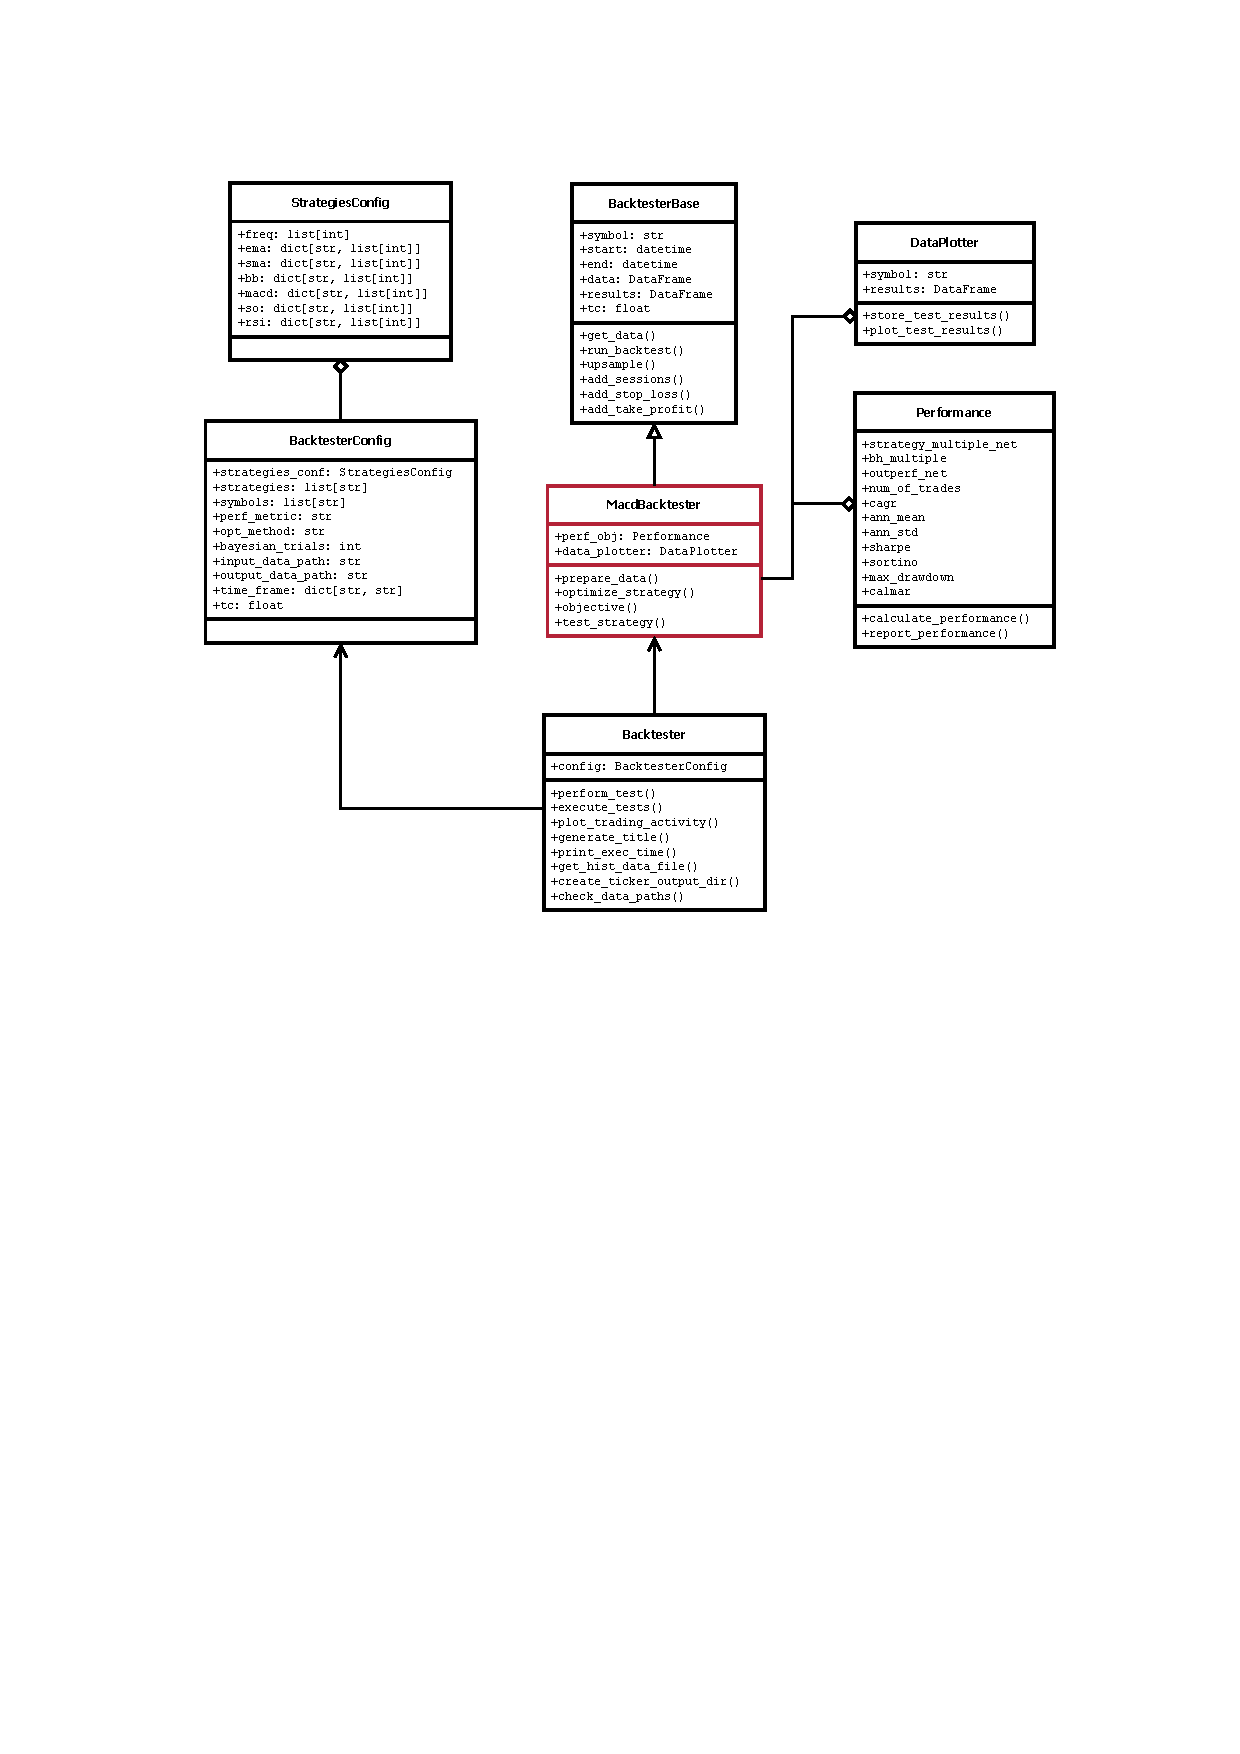
\includegraphics[page=1, trim=30mm 135mm 0 25mm, width=1.1\textwidth, clip]{./pdf/backtester_uml.pdf}
\caption{Technical indicator based backtesting architecture.}
\label{fig:tech_indicator_arch}
\end{figure}

\noindent
Technical indicators are mathematical calculations based on historical price, volume, or open interest information that aim to predict future price movements.
Commonly used in technical analysis, these indicators provide insight into the market's direction, strength, momentum, and volatility.

The cornerstone of this framework lies in its automated, vectorized backtesting, which furnishes a remarkably efficient backtesting utility.
The framework incorporates two distinct backtesting variations: one for machine learning-based models and another for technical indicator-based models.
A notable feature of the framework is its extensibility; new testing algorithms can be seamlessly incorporated and configured.
For integration, each new algorithm should inherit from the \texttt{BacktesterBase} class, located in the \texttt{backtester\_base.py} module.
Furthermore, they must implement the methods: \texttt{prepare\_data}, \texttt{optimize\_strategy}, \texttt{objective()}, and \texttt{test\_strategy()}.

Figure \ref{fig:tech_indicator_arch} delves into the architecture of the technical indicator-based backtesting component within the framework.
Notably, the UML class (delineated in red) titled \texttt{MacdBacktester} is a descendant of the \texttt{BacktesterBase} class.
This base class equips all models with essential methods such as \texttt{get\_data}, \texttt{run\_backtest}, \texttt{add\_stop\_loss}, and \texttt{add\_take\_profit}, to name a few.
Additional classes, namely \texttt{DataPlotter} and \texttt{Performance}, are harnessed to compute and graphically represent performance metrics for each test.

A pivotal aspect of this framework is the adaptability of each algorithm's parameters.
Users have the flexibility to configure the parameter spaces via the JSON file named \texttt{backtesterconfig}.
This configuration is subsequently ingested and validated through \texttt{pydantic}.
For optimization, users can employ either the grid search method or the Bayesian method.
While grid search explores all possible combinations in the parameter space, the Bayesian approach uses probability distributions to improve the search.
Given the configuration of parameter spaces for each algorithm, numerous combinations---potentially tens of thousands---can be tested for each symbol.
The performance results for all these combinations are consolidated into a single CSV file, facilitating subsequent analysis.

Consider the snapshot below, extracted from a more intricate configuration, as a case in point:

\begin{lstlisting}[style=jsonstyle, caption={Machine Learning Pipeline Configuration}]
{
  "opt_method": "bayesian",
  "bayesian_trials": 1500,
  "time_frame": {
    "start_date": "",
    "end_date": "2022-12-31 23:59:00"
  },
  "symbols": ["XRPUSDT", "LTCUSDT", "TRXUSDT"],
  "strategies_config":
  {
    "freq" : [5, 125, 5],
    "ema": {
       "ema_s": [6, 60, 4],
       "ema_l": [10, 200, 5]
    }
  }
}
\end{lstlisting}

Furthermore, individual backtesting results for each symbol and strategy can be visualized, as depicted in fig.~\ref{fig:backtest_results}.
This figure showcases the performance results of the optimized strategy juxtaposed against the buy-and-hold strategy.
As an illustrative example, the EMA strategy for LTCUSDT is spotlighted. All pertinent parameters are illustrated above the primary plot.
Testing was executed on historical data spanning from 2021-01-01 to 2021-12-31.

\begin{figure} [H]
\centering
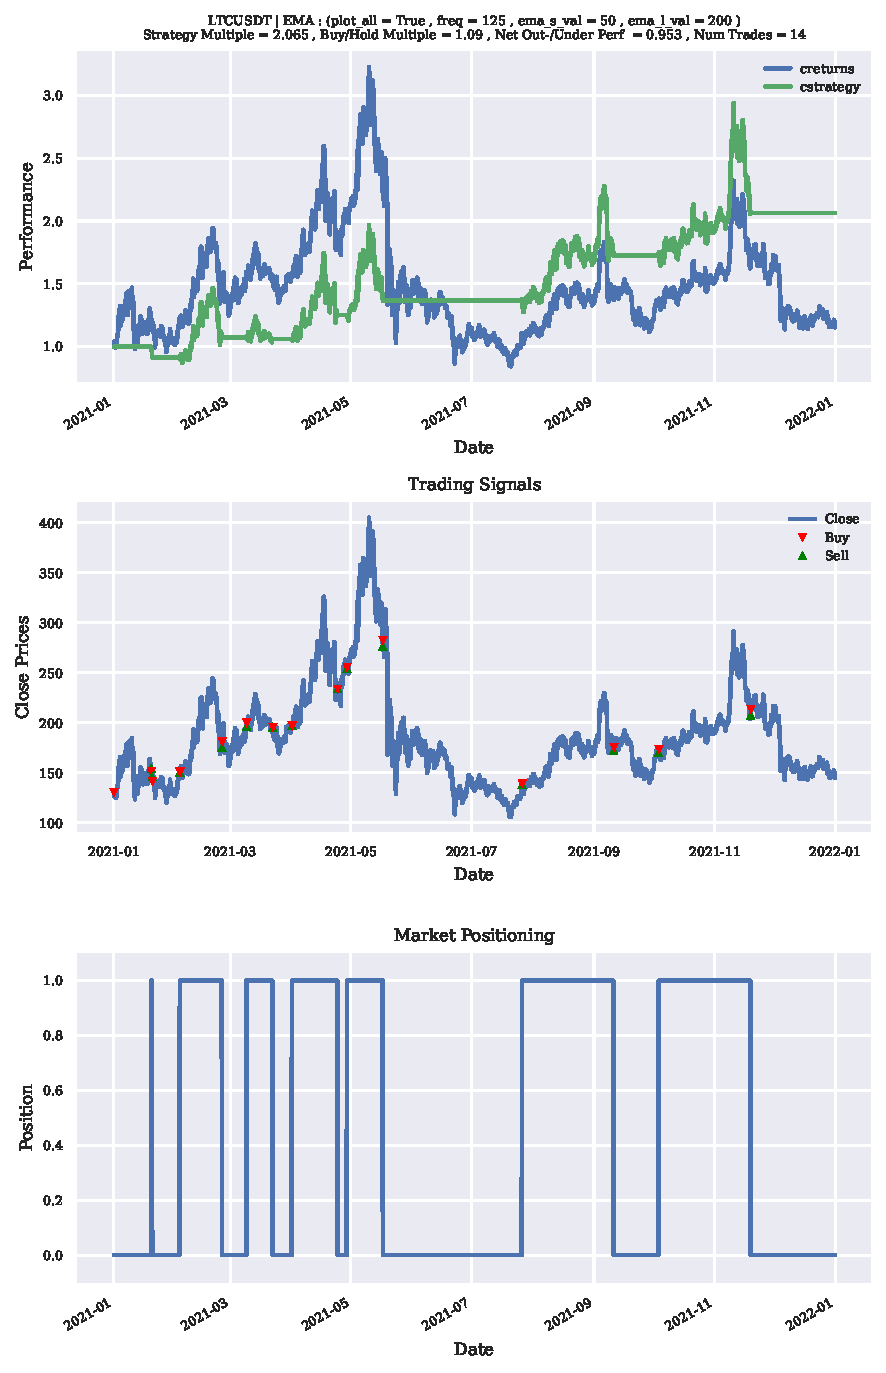
\includegraphics[page=1, trim=0mm 0mm 0 0mm, width=0.95\textwidth, clip]{./pdf/backtesting_results.pdf}
\caption{Results of Backtesting of MACD Stragegy of XRPUSDT.}
\label{fig:backtest_results}
\end{figure}

The secondary plot, detailing close prices, accentuates the drastic price fluctuations during this period.
Impressively, the algorithm managed to surpass the buy-and-hold strategy, achieving an outperformance of 0.953 (which can be construed as a 95\% enhancement).
Furthermore, individual backtesting results for each symbol and strategy can be visualized, as depicted in fig.~\ref{fig:backtest_results}.

\begin{table}[H]
    \centering
    \begin{tabular}{l}
        \texttt{LTCUSDT | EMA : (freq = 125 , ema\_s\_val = 50 , ema\_l\_val = 200 )} \\
        \texttt{Strategy Multiple = 2.065 , Buy/Hold Multiple = 1.09 ,} \\
        \texttt{Net Out-/Under Perf = 0.953 , Num Trades = 14} \\
    \end{tabular}
\end{table}
This figure showcases the performance results of the optimized strategy juxtaposed against the buy-and-hold strategy.
As an illustrative example, the EMA strategy for LTCUSDT is spotlighted. All pertinent parameters are illustrated above the primary plot.
Testing was executed on historical data spanning from 2021-01-01 to 2021-12-31.
The secondary plot, detailing close prices, accentuates the drastic price fluctuations during this period.
Impressively, the algorithm managed to surpass the buy-and-hold strategy, achieving an outperformance of 0.953 (which can be construed as a 95\% enhancement).
% trim={<left> <lower> <right> <upper>}
%\vspace{-2cm}


%Parameters:
%{'algorithm': 'SAMME', 'base_estimator': None, 'learning_rate': 0.5, 'n_estimators': 100, 'random_state': None}







  % Overview of the main backtesting directory
\input{indicators.tex}  % Indicators
\chapter{Machine Learning based Backtesting}

In the world of machine learning (ML), classification is about sorting things into categories. When applied to trading, ML Models predict whether the price will go up or down based on today's as well as historical data.
Using ML to predict trading outcomes requires a systematic approach.
This structured process is visualized as a pipeline, detailed in fig. \ref{fig:ml_pipeline}.

%trim=left bottom right top,
\section{ML Trading Pipeline}


\begin{figure}[H]
\centering
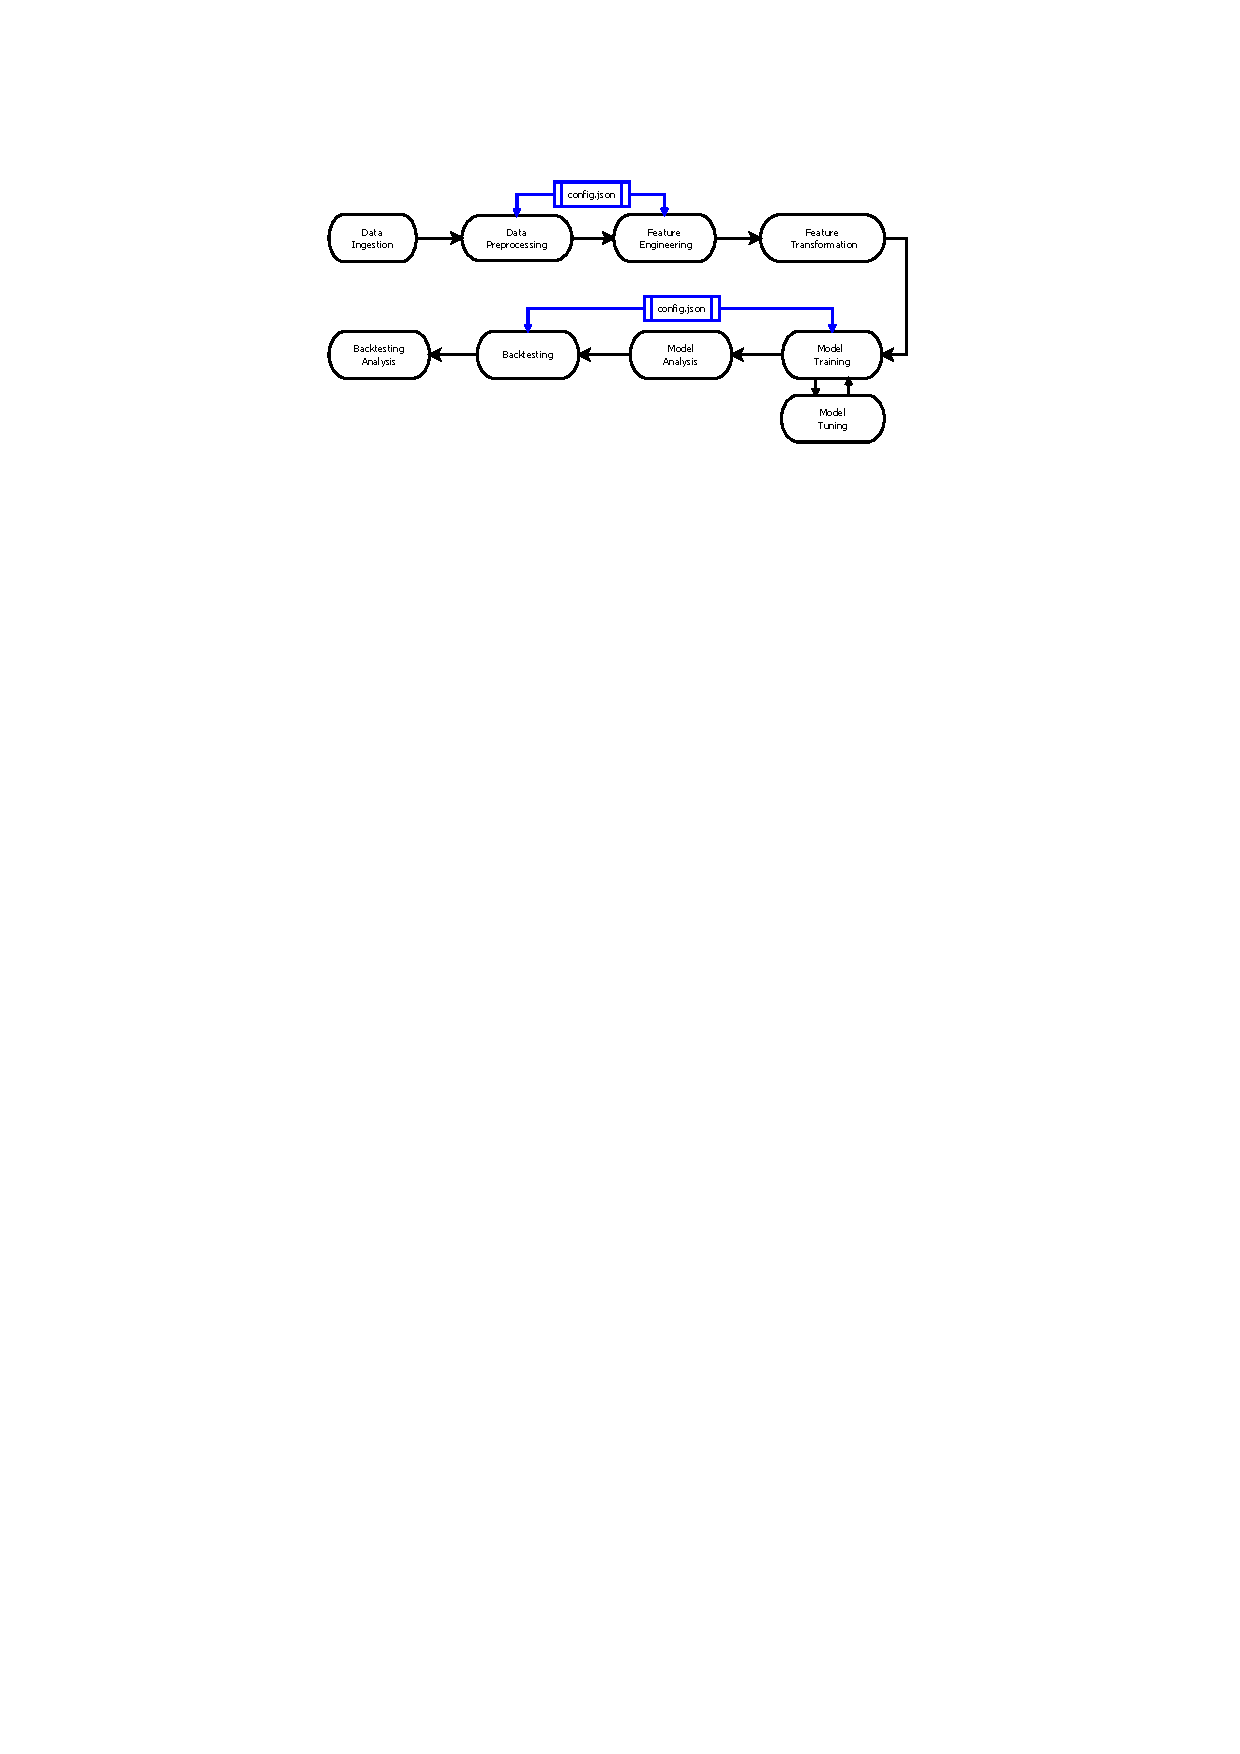
\includegraphics[trim=25mm 220mm 55mm 30mm, width=1.2\textwidth, clip]{./pdf/ml_pipeline.pdf}
\caption{Machine Learning Trading Pipeline: A visualization of the process, detailing steps from data acquisition and preprocessing, feature engineering and transformation, model training and optimizing, to the final execution and evaluation of trades based on model predictions.}
\label{fig:ml_pipeline}
\end{figure}

This pipeline initiates with raw historical data sourced from Binance and advances through a series of steps
leading to informed trading decisions. The process involves backtesting using the trained and optimized ML model on the historical data.
The pipeline steps can also be executed independently.
For instance, starting with data ingestion and preprocessing can be followed by feature engineering and data visualization to gain a deeper understanding of the dataset. The steps of the pipeline in  fig. \ref{fig:ml_pipeline}. are detailed in the subsequent subsections.

\subsection{ML Trading Pipeline Configuration}
The following JSON configuration in lst. \ref{lst:pipeline_conf} is used to set up the machine learning pipeline.
The \texttt{dataset\_conf} element specifies details such as the cryptocurrency symbol to be backtested (BTCUSDT in this case), the frequency of the time series data, and the start and end dates. Additionally, it offers an option to set the date for splitting the dataset into training and test sets.
The configuration also includes options to set the desired model and specify the parameter ranges. This enables fine-tuning via grid search for the selection of optimal parameters.
Also the \texttt{target\_conf} element allows for the selection of the target for the classification model. There are several target variants to choose from, that are describe later.




\begin{lstlisting}[style=jsonstyle, caption={Machine Learning Pipeline Configuration},  captionpos=b, label=lst:pipeline_conf][h]
{
  "tc": 0.001,
  "dataset_conf": {
     "symbol": "BTCUSDT",
     "freq": "1d",
     "start_date": "2018-01-01 00:00:00",
     "end_date": "2023-08-30 23:59:00",
     "split_date": "2022-12-31 23:59:00",
     "mode": "full",
     "target_conf": {
       "target": "Exceed_Avg_Returns"
    }
  },
  "model_name": "RandomForestClassifier",
  "model_type": "classification",
  "models_config": [
     {
       "model": "AdaBoostClassifier",
       "params": {
          "n_estimators": [10, 30, 100],
          "learning_rate": [0.01, 0.1, 1.0],
          "algorithm": ["SAMME", "SAMME.R"]
       }
     }
  ]
}
\end{lstlisting}



\subsection{Data Ingestion and Preprocessing}
The first step involves ingesting the data required for backtesting. This data can be sourced from Binance using the \texttt{data\_retrieve.py} module, as detailed in the previous chapter.
The data is saved in the \texttt{historical\_data} folder, which is located within the corresponding symbol's subfolder, created during the data download process.
Once the data has been retrieved, it can be ingested into the pipeline. It's recommended to retrieve data with a one-minute time bar length,
as this can be efficiently downsampled later for larger intervals such as an hour or a day.
This is done during the data preprocessing phase. The ingested data is downsampled based on the bar length specified in the configuration (refer to \lstinline[label=lst:pipeline_conf]{lst:pipeline_conf}, line 5), where the \texttt{freq} parameter is set to \texttt{1d}.
Furthermore, a validation check is run to ensure data integrity.

%\vspace{20mm} % Put space between figure and subsection title
%\vspace{10mm} % Adjust the value to your liking
\FloatBarrier % This ensures that the figure is placed before continuing with the subsequent content
\subsection{Feature Engineering}
Feature engineering is a critical step in improving the model's predictive capability.
The goal is to identify features that could potentially influence the model's performance.
Technical indicators are utilized to create features that help models predict upcoming price movements based on historical market data.
The technical indicators used in the \texttt{ml\_feature\_engineer} module can be broadly categorized into momentum-based, trend-based, and volume-based.


\begin{itemize}
    \item \textbf{Momentum-based Indicators:} These are primarily concerned with the speed of price movements. Features like Rate of Change (ROC), Momentum, variations of the Stochastic Oscillator, and the Relative Strength Index (RSI) fall into this category.

    \item \textbf{Trend-based Indicators:} Aimed at identifying the movement direction over time, these include indicators such as the Moving Average (MA) and the Exponential Moving Average (EMA).

    \item \textbf{Volume-based Indicators:} Volume, in trading, refers to the number of shares or contracts traded in a security or market. The feature set for this category includes the On-Balance Volume (OBV).
\end{itemize}

\begin{lstlisting}[style=pythonstyle, language=Python, caption={Function to add features to the dataset},  captionpos=b, label=lst:add_features_function]
def add_features(self):
    """Add various technical indicators to the dataset."""
    for n in self.periods:
        self._add_ma(n)
        self._add_ema(n)
        self._add_rsi(n)
        self._add_sto(n)
        self._add_mom(n)
        self._add_roc(n)
        self._add_stos(n)
        self._add_stomom(n)
        self._add_storoc(n)
        self._add_stoch_rsi(n)
        self._add_sto_cross(n)
    self._add_obv()
    self._add_returns()
    self._add_rolling_cum_returns()
    self._add_rolling_cum_range()
    self._add_day_of_week()
    self._calculate_range()

\end{lstlisting}


Following this, a target is computed, which can also be specified in the configuration file. The available target variants include:
\begin{itemize}
    \item \textbf{Simple}: Predicts if the next day's price will go up or down based on today's closing price.
    \item \textbf{MA\_Relative}: Checks if today's closing price is above its short-term average and rising.
    \item \textbf{Momentum}: Examines if the stock's momentum is positive and increasing.
    \item \textbf{ROC}: Looks at if the rate of change (ROC) is positive and on the rise.
    \item \textbf{Consecutive\_Increases}: Predicts if returns will rise for the third consecutive time after a decline.
\end{itemize}

\begin{figure}[h]
\centering
\begin{adjustbox}{max width=1\textwidth,center}
    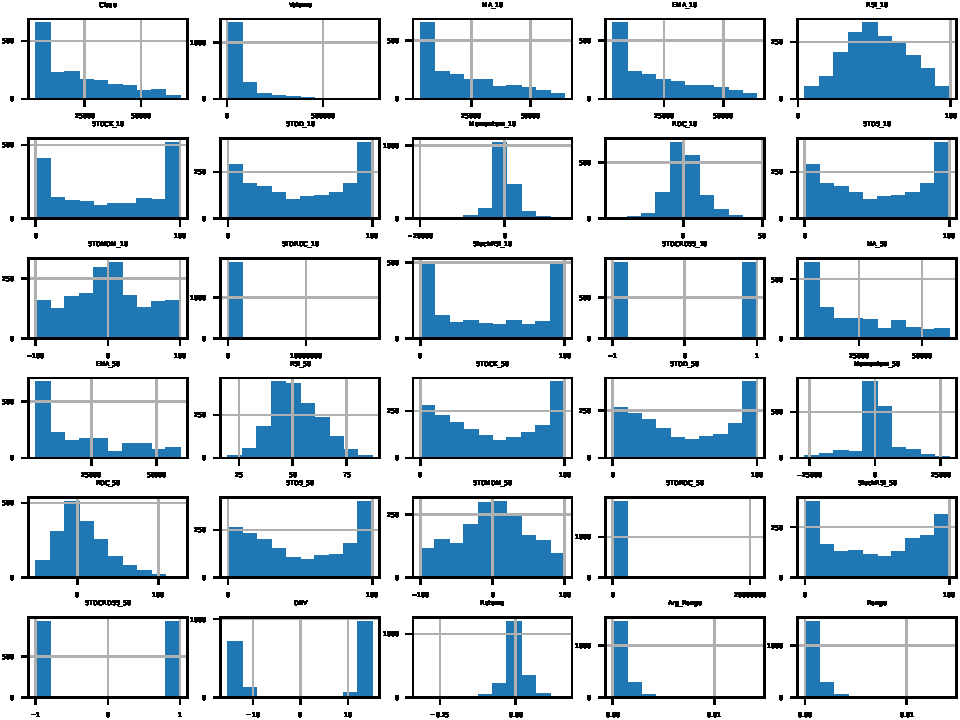
\includegraphics[scale=1]{./pdf/dataset_histogram.pdf}
\end{adjustbox}
\caption{Histogram of engineered features from the BTCUSDT historical data.}
\label{fig:dataset_histogram}
\end{figure}

 %Confusion matrix (left) presenting actual versus predicted values, alongside key performance metrics (right) indicating the model's accuracy, precision, recall, and F1 score.}
\subsection{Feature Transformation}

After engineering the features, it's essential to transform them to meet the specific requirements of machine learning models. Many algorithms have assumptions about the data's scale and distribution.
Hence, features undergo transformations using techniques like \texttt{Standardization} and {MinMax Scaling}.

It's importan to apply the same transformations with according parameters, to both the training and testing datasets or any new incoming data. This ensures consistent and accurate model predictions.

The entire transformation workflow, from data loading, preprocessing, to feature-related operations, is orchestrated by the \texttt{DataManager} and \texttt{FeatureEngineer} classes (fig. \ref{fig:dataManagerFeatureEngineer}).



\subsection{Data Visualization}
For data analysis the \texttt{ml\_model\_evaluator} module was implemented with appropriate methods. It provides tools for both data and model checks.
The prepared data can be visualized in various ways, including target distributions, feature covariance matrices, and feature histograms.

The \textbf{distribution of the predicted variable} across both training and validation datasets is showed in fig. \ref{fig:signal_distribution}.
Notably, the distribution between the two classes (1's and 0's) is nearly balanced in both datasets. Such a balanced distribution is crucial for training machine learning models effectively, ensuring that they aren't biased towards one class.

\begin{figure}[h]
\centering
\begin{adjustbox}{max width=1\textwidth,center}
    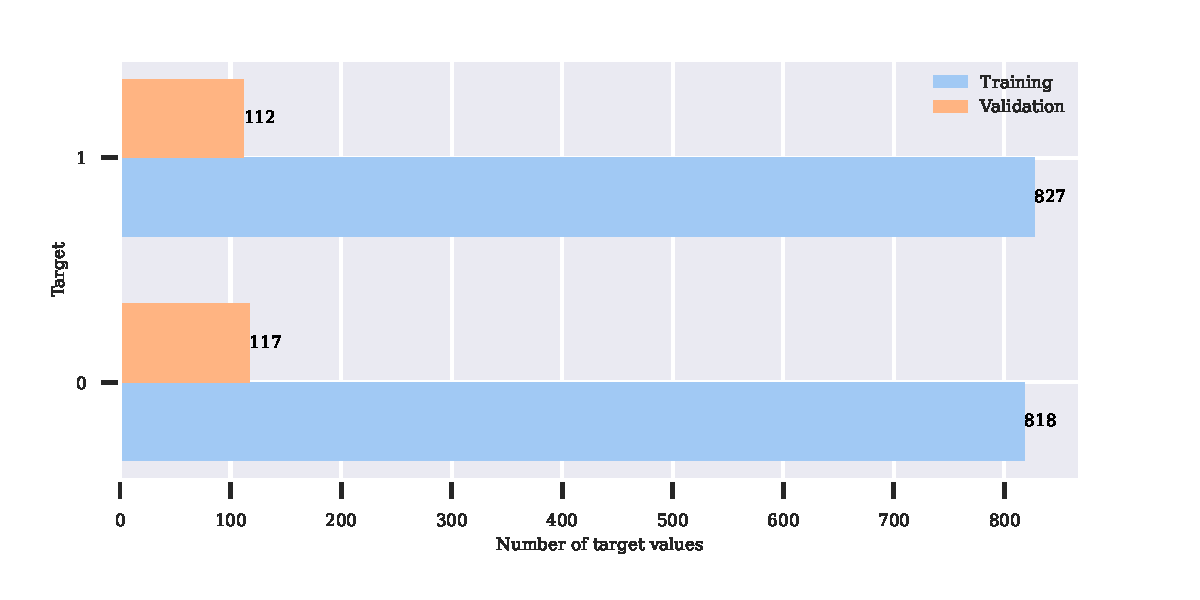
\includegraphics[scale=1]{./pdf/report/sig_distr.pdf}
\end{adjustbox}
    \caption{The distribution of target values in both the training testing datasets.}
\label{fig:signal_distribution}
\end{figure}

The fig. \ref{fig:corr_coef} illustrates the \textbf{correlation coefficients} between various feature variables in the dataset.
Each cell in the matrix represents the degree of correlation between two features: a value close to 1, represented by dark green, signifies a strong positive correlation, while a value close to -1, shown in white, indicates a strong negative correlation.

%trim=left bottom right top,
\begin{figure}[h]
\centering
\begin{adjustbox}{max width=1.2\textwidth,center}
    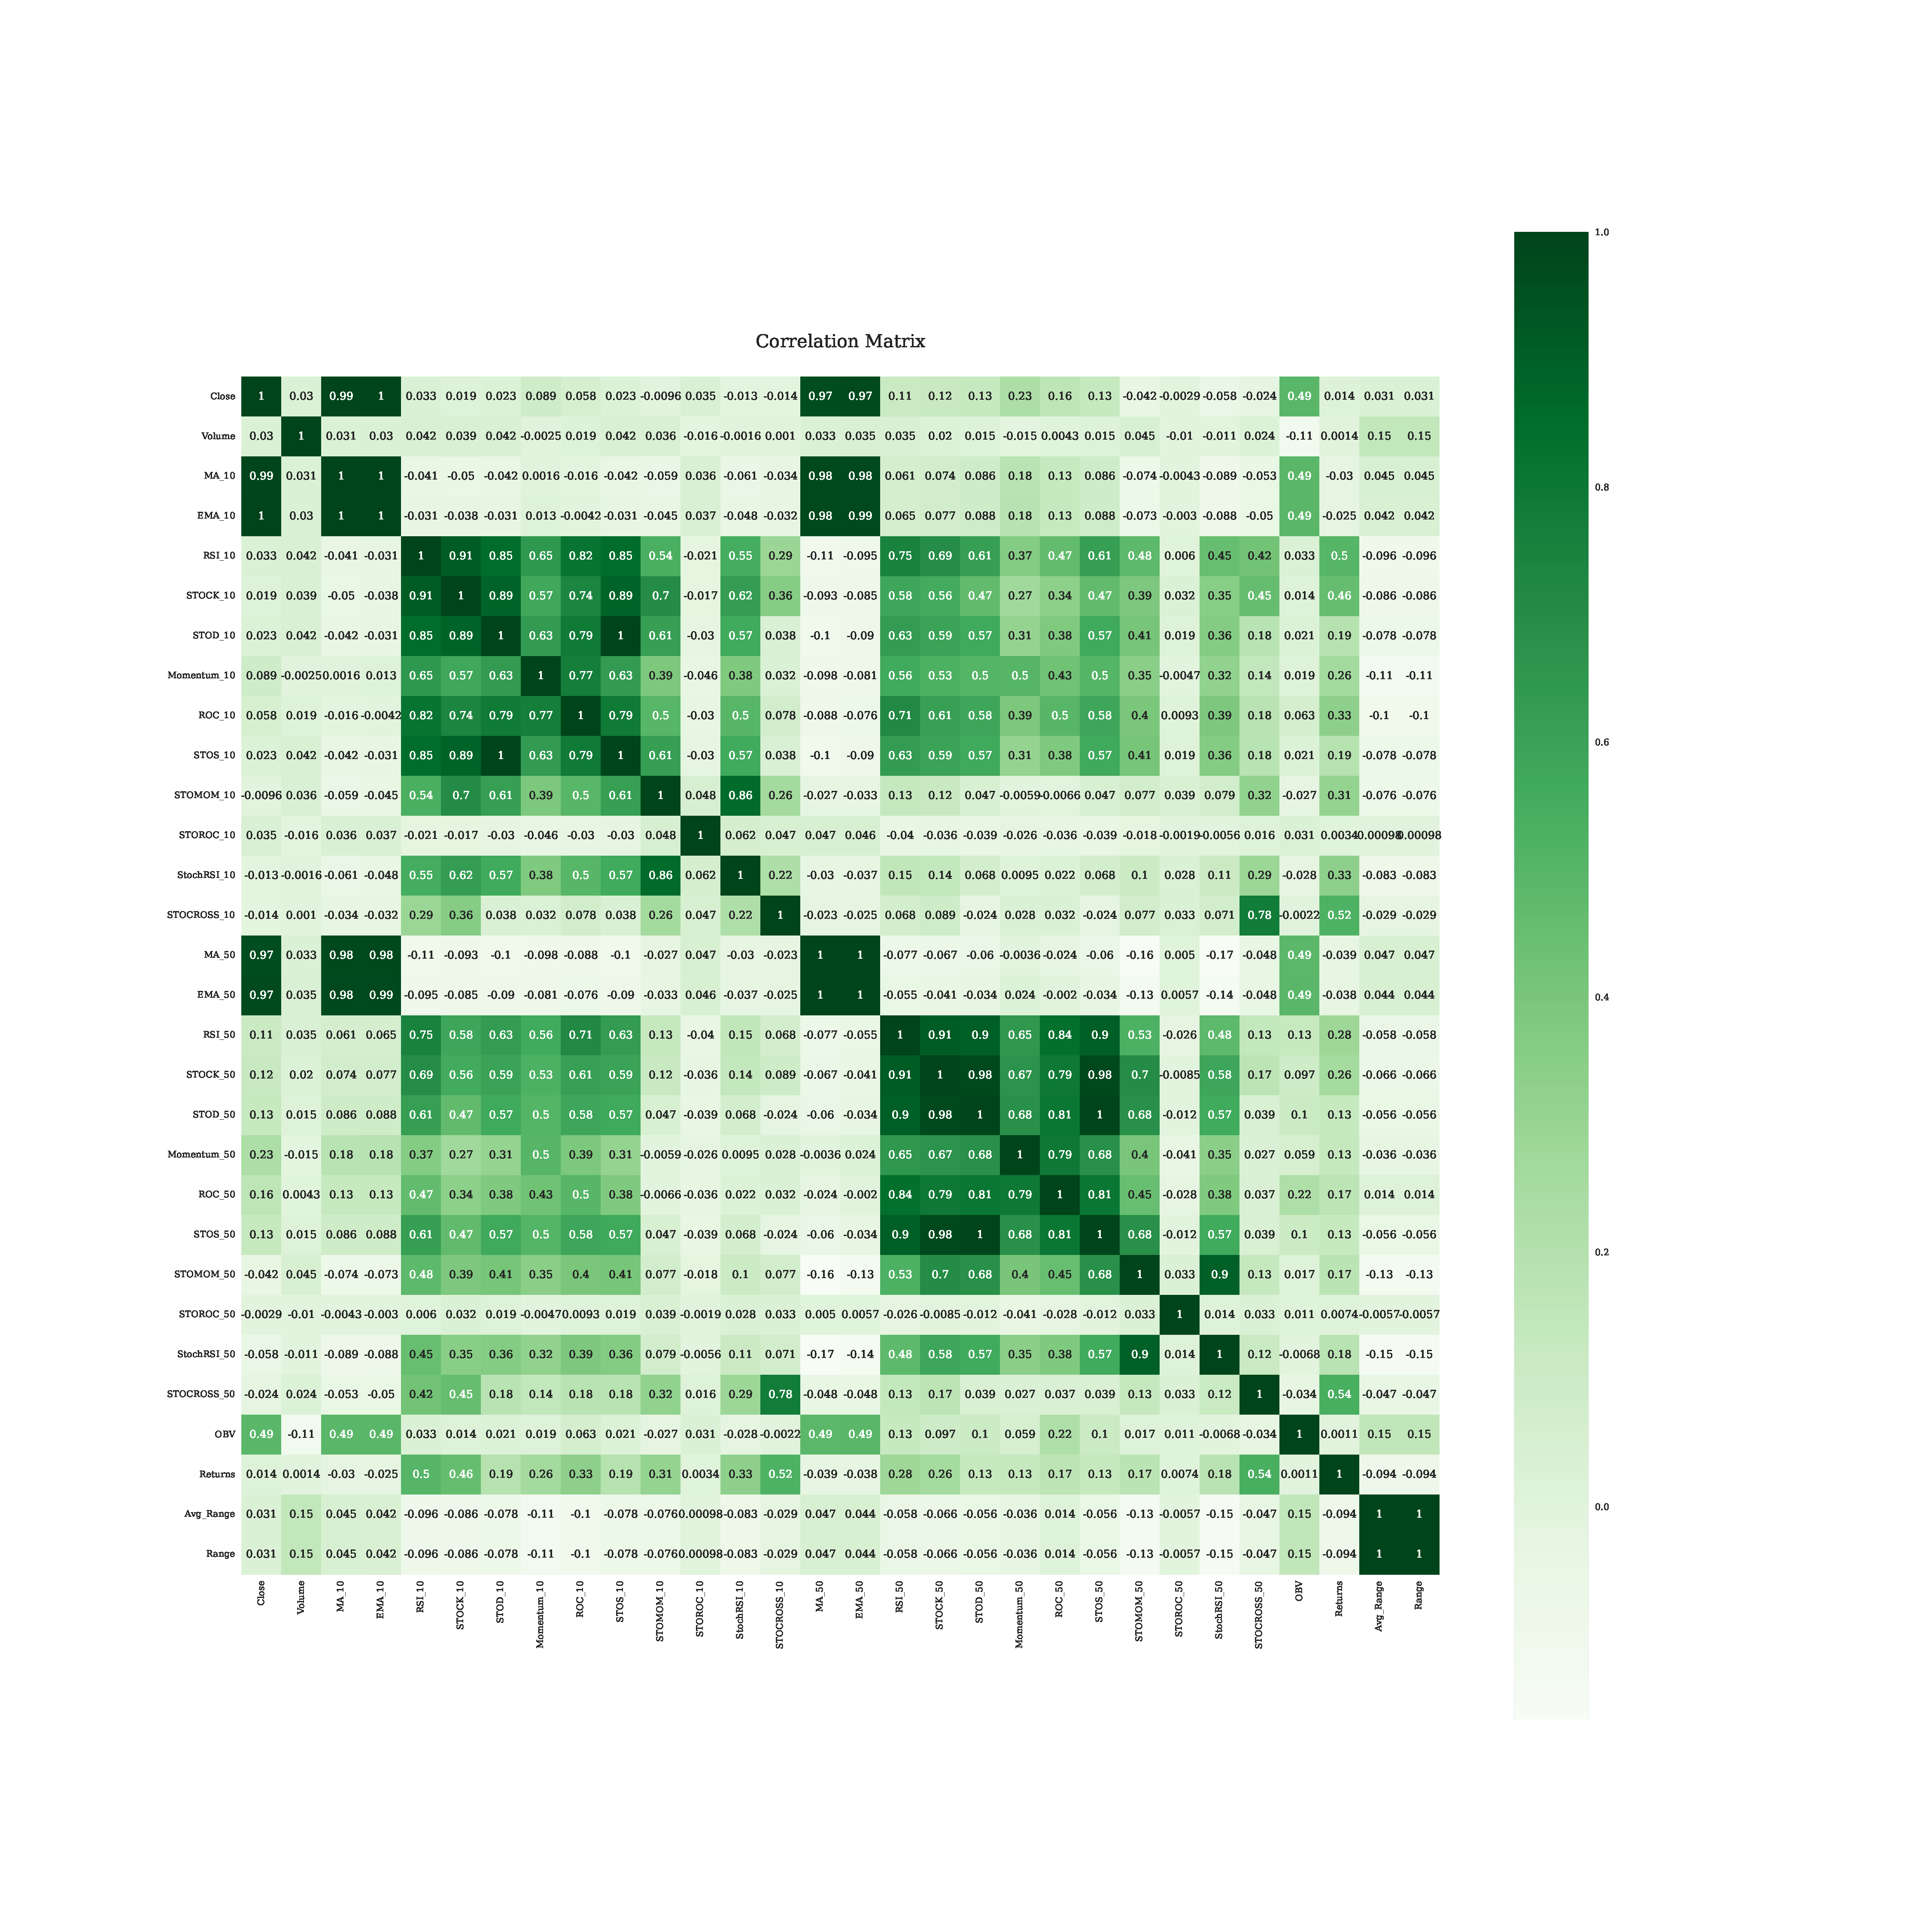
\includegraphics[scale=1.2, trim={30mm 70mm 50mm 110mm}, clip]{./pdf/correlation_matrix.pdf}
\end{adjustbox}
\caption{Correlation Coefficient between features variables.}
\label{fig:corr_coef}
\end{figure}

The fig. \ref{fig:dataset_histogram} presents a \textbf{histogram} showcasing the distribution of engineered features derived from the BTCUSDT historical data. Each bar in the histogram represents the frequency of occurrences for a particular value or range of values. This visualization provides insights into the distribution patterns and potential skewness of the different features in the dataset.



\subsection{Model Training and Optimization}
The logic for model training and backtesting is encapsulated within the \texttt{ml\_backtester.py} module,
while the \texttt{ml\_optimizer.py} module is dedicated to optimization purposes, as depicted in Figure \ref{fig:<your_figure_label_here>}.
The \texttt{\_optimize\_model} function in the \texttt{ml\_backtester.py} module is responsible for the model optimization process.
It utilizes the instance of the MlOptimizer class to perform searching for the best parameters of the model using techniques such as Grid Search with Cross-Validation.
In a grid search, a grid of all possible hyperparameter combinations is created, and the model is trained using each one of them. The best model is then used in the \texttt{\_generate\_predictions}
function to predict the trends in price movements on unseen data. Once optimized, the trained model specific to a cryptocurrency can be saved for subsequent use and reloaded as needed.
Model specifics, such as the model type (for instance, AdaBoostClassifier) and its hyperparameter ranges, are defined in the JSON configuration file (see lst. \ref{lst:pipeline_conf}).

\begin{lstlisting}[style=pythonstyle, language=Python, caption={Function of MlBacktester class for model optimization and predictions.},  captionpos=b, label=lst:add_features_function]
def _optimize_model(self):
   # Instantiate the GridSearchOptimizer
   optimizer = GridSearchOptimizer(self.data_manager.X_train,
                                self.data_manager.y_train,
                                self.config.dataset_conf.symbol,
                                task_type=self.config.model_type,
                                num_folds=self.config.num_folds,
                                scoring=self.config.scoring)

   # Optimize the model using configured parameters grid
   best_model = optimizer.grid_search(self.config.model_name,
                                  self.model,
                                  self.get_model_params_grid())

   # Update the model of the strategy to the optimized model
   self.model = best_model

def _generate_predictions(self):
   '''Generate predictions using the model.'''
   predictions = self.model.predict(self.data.X_train)
   self.data['predictions'] = predictions
   self.data['predictions'].ffill().fillna(0, inplace=True)

\end{lstlisting}

\subsection{Model Evaluation using Classification Metrics}
After training the trading model's performance can be evaluated using several metrics. These metrics provide insights into the model's predictions and highlight potential areas for improvement.
The performance data for both the training and testing of the model are visualized in fig. \ref{fig:conf_matrix}.
For each phase (training and testing):

The left diagram presents the confusion matrix, which shows the number of correct and incorrect predictions made by the model.
The right diagram visualizes key performance metrics, specifically: accuracy, precision, recall, and F1 score. Each metric is also further described in  more detail below.
\begin{figure}[h]
    \centering

    \begin{subfigure}[b]{\textwidth}
        \begin{adjustbox}{max width=0.8\textwidth,center}
            \includegraphics[scale=0.8]{./pdf/report/report\_train.pdf}
        \end{adjustbox}
        \caption{Model Performance Metrics based on Training Data.}
        \label{fig:train_perf}
    \end{subfigure}

    \bigskip % Adds some vertical space between the two subfigures

    \begin{subfigure}[b]{\textwidth}
        \begin{adjustbox}{max width=0.8\textwidth,center}
            \includegraphics[scale=0.8]{./pdf/report/report\_test.pdf}
        \end{adjustbox}
        \caption{Model Performance Metrics based on Testing Data.}
        \label{fig:test_perf}
    \end{subfigure}

    \caption{Visualization of the Classification Report.}
    \label{fig:conf_matrix}
\end{figure}

\begin{itemize}
	\item \textbf{True Positive:} Represents the number of times the model correctly predicted an upward trend and the price actually went up.

	\item \textbf{True Negative:} Represents the number of times the model correctly predicted a downward trend and the price actually went down.

	\item \textbf{False Positive:} Represents the number of times the model incorrectly predicted an upward trend and the price went down or stayed the same. This type of error could result in a missed shorting opportunity or a loss if one decided to buy in Long Only strategies.

	\item \textbf{False Negative:} Represents the number of times the model incorrectly predicted the downward trend and the price went up or stayed the same. This type of error could result in missed profit opportunities from not buying.

	\item \textbf{Recall:} The ratio of the number of correct positive predictions (TP) to the total actual positives (TP + FN). In mathematical terms, Recall $= \frac{TP}{TP + FN}$. In trading, it indicates how well the model identifies actual upward movements. A high recall means the model captures most of the upward trends, but this can also be achieved at the expense of more false positives.

	\item \textbf{Precision:} The ratio of correct positive predictions (TP) to the total predicted positives (TP + FP). In mathematical terms, Precision $= \frac{TP}{TP + FP}$. Shows how many of the predicted upward trends by the model were actually correct. High precision means that when the model predicts an upward trend, it's likely correct. But a higher precision might come at the expense of missing some actual upward trends (lower recall).

	\item \textbf{Accuracy:} The ratio of correct predictions (both TP and TN) to the total number of predictions (TP + TN + FP + FN). In mathematical terms, Accuracy $= \frac{TP + TN}{TP + TN + FP + FN}$. In trading, it gives an overall measure of how often the model is correct, regardless of whether it's predicting upward or downward movement.

	\item \textbf{F1 Score:} The harmonic mean of precision and recall, providing a balance between the two. It is given by the formula: F1 $= 2 \times \frac{\text{Precision} \times \text{Recall}}{\text{Precision} + \text{Recall}}$. It's especially useful when the class distribution is imbalanced. In trading, a high F1 score suggests the model has a balanced performance in terms of identifying upward trends and avoiding false alarms.
\end{itemize}


\subsection{Backtesting and Analysis}
After the model is trained and fine-tuned, it's crucial to check how good it is by testing its effectiveness not just on the basis of typical classification metrics but also on how well it performs in a simulated trading environment.

The code listing \ref{lst:add_features_function} showcases the \texttt{run\_strategy} function, a part of the \texttt{MlBacktester} class. This function is designed to run the backtesting process:

\begin{figure}[h]
\centering
\begin{adjustbox}{max width=1.3\textwidth,center}
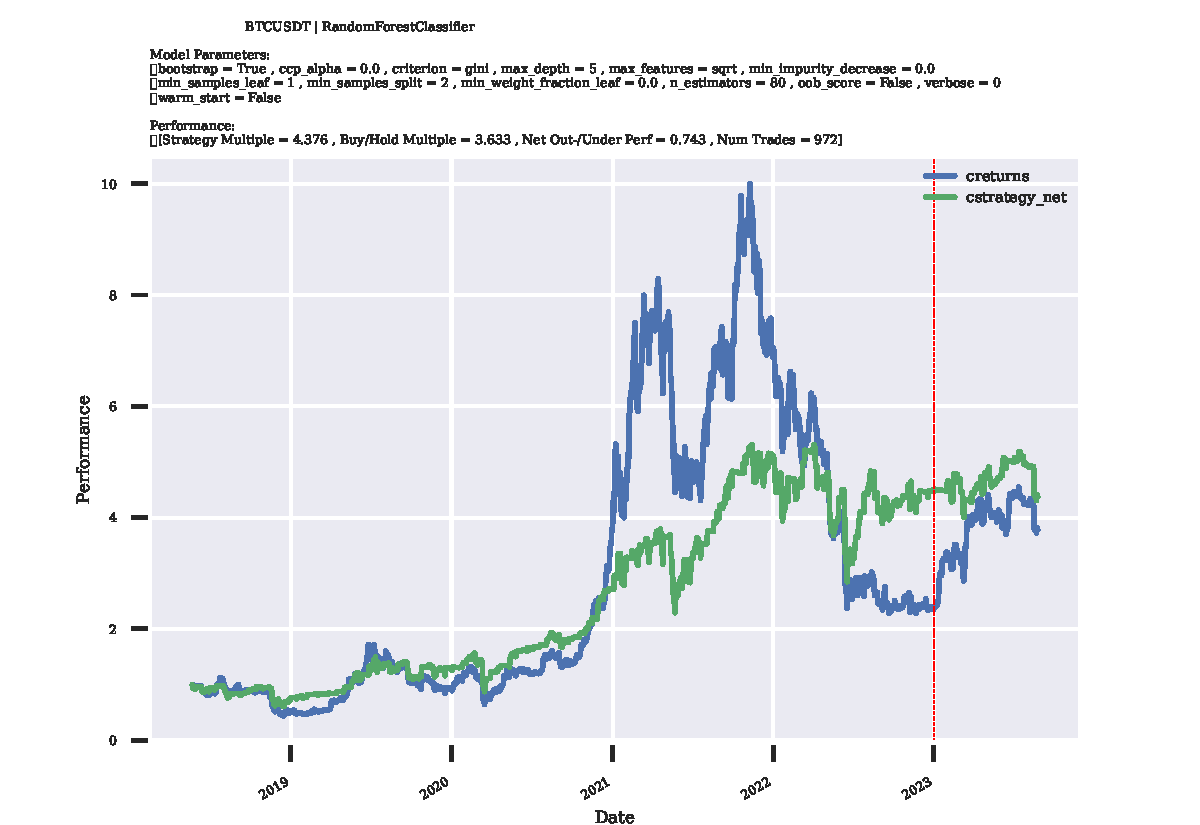
\includegraphics[scale=1.3]{./pdf/report/backtest_res.pdf}
\end{adjustbox}
\caption{Feature Significance in Model Prediction}
\label{fig:backtest_res}
\end{figure}

After generating predictions, the strategy values are calculated. These strategy values reflect the positions the model would take based on its predictions.
Further, trades are determined and adjustments are made to account for transaction costs, which are often overlooked but can significantly impact net returns in real-world scenarios.
Finally, cumulative metrics are computed, followed by a performance evaluation to assess the overall success of the trading strategy.
By summing the strategy returns, the model's hypothetical profitability over the backtesting period is determined.

\begin{lstlisting}[style=pythonstyle, language=Python, caption={\vspace*{1cm}Function of MlBacktester class for backtesting execution.},  captionpos=b, label=lst:add_features_function]
def run_strategy(self):
    '''Backtests the trading strategy.'''
    self._generate_predictions()
    self._calculate_strategy_values()
    self._calculate_trades()
    self._adjust_for_transaction_costs()
    self._calculate_cumulative_metrics()
    self.perf_evaluator._calculate_perf(self.data)

\end{lstlisting}

A common benchmark to assess the strategy's success is the "buy and hold" method.
In this approach, the asset is bought and kept throughout the entire period without incurring extra costs or decisions based on price changes.
Comparing the total strategy returns to the "buy and hold" method's returns provides an understanding of the ML-based strategy's added benefit.
If the model outperformes this benchmark, it can be considered as useful for trading.

The fig. \ref{fig:backtest_res} illustrates the comparison between the returns of the "buy and hold" strategy and those of the configured \texttt{AdaBoostClassifier} model's strategy.
The model's strategy achieved a return multiple of 4.376. This surpasses the 3.633 return from the "buy and hold" method, resulting in a net outperformance of 0.743, or 74.3\%.
This outperformance is observed at the end of the backtesting period, which can also be configured in the JSON configuration shown in lst. \ref{lst:pipeline_conf}.
Moreover, the analysis took into account Binance's trading fees of 0.1\% for spot trading, ensuring a more realistic representation of potential real-world returns.
The backtesting results show the potential of the model for real-world trading scenarios.





\begin{figure}
\centering
\begin{adjustbox}{max width=1.2\textwidth,center}
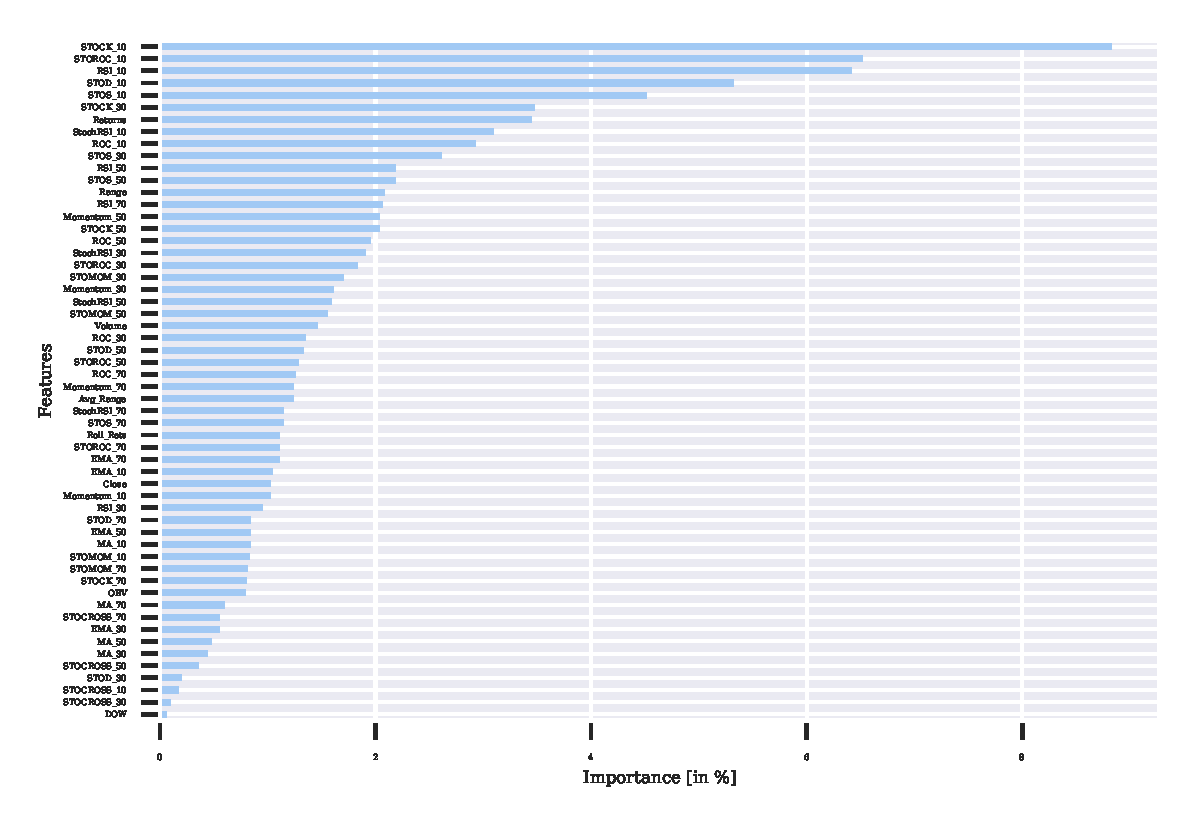
\includegraphics[scale=1.2]{./pdf/report/feature_importance.pdf}
\end{adjustbox}
\caption{Feature Significance in Model Prediction}
\label{fig:feature_importance}
\end{figure}


\begin{figure}[h]
\centering
\includegraphics[width=0.9\textwidth]{./pdf/report/explained\_variance.pdf}
\caption{Explained Variance of Features after Performing Feature Reduction.}
\label{fig:explained_variance}
\end{figure}
  % ML Backtesting
%
\begin{figure}[h]
\dirtree{%
.1 backtester.
.2 historical\_data.
.3 BTCUSDT
.3 ETHUSDT
.3 \ldots.
.2 \ldots.
.2 utilities.
.3 credentials.py.
.3 data\_plot\_ml.py.
.3 logger.py.
.3 performance.py.
.3 report\_email.py.
.3 data\_utils.
.4 data\_loader.py.
.4 data\_manager.py.
.4 data\_retriever.py.
.4 ml\_data\_manager.py.
.4 ml\_feature\_engineer.py.
.3 {\textbf{plot\_utils}}.
.4 {\textbf{backtesting\_plotter.py}}.
.4 {\textbf{ml\_model\_evaluator.py}}.
}

\caption{Directory structure of the project.}\label{fig:projectStructure}
\end{figure}  % Vectorized Backtesting

\chapter{Deployment}


\begin{figure}[H]
\centering
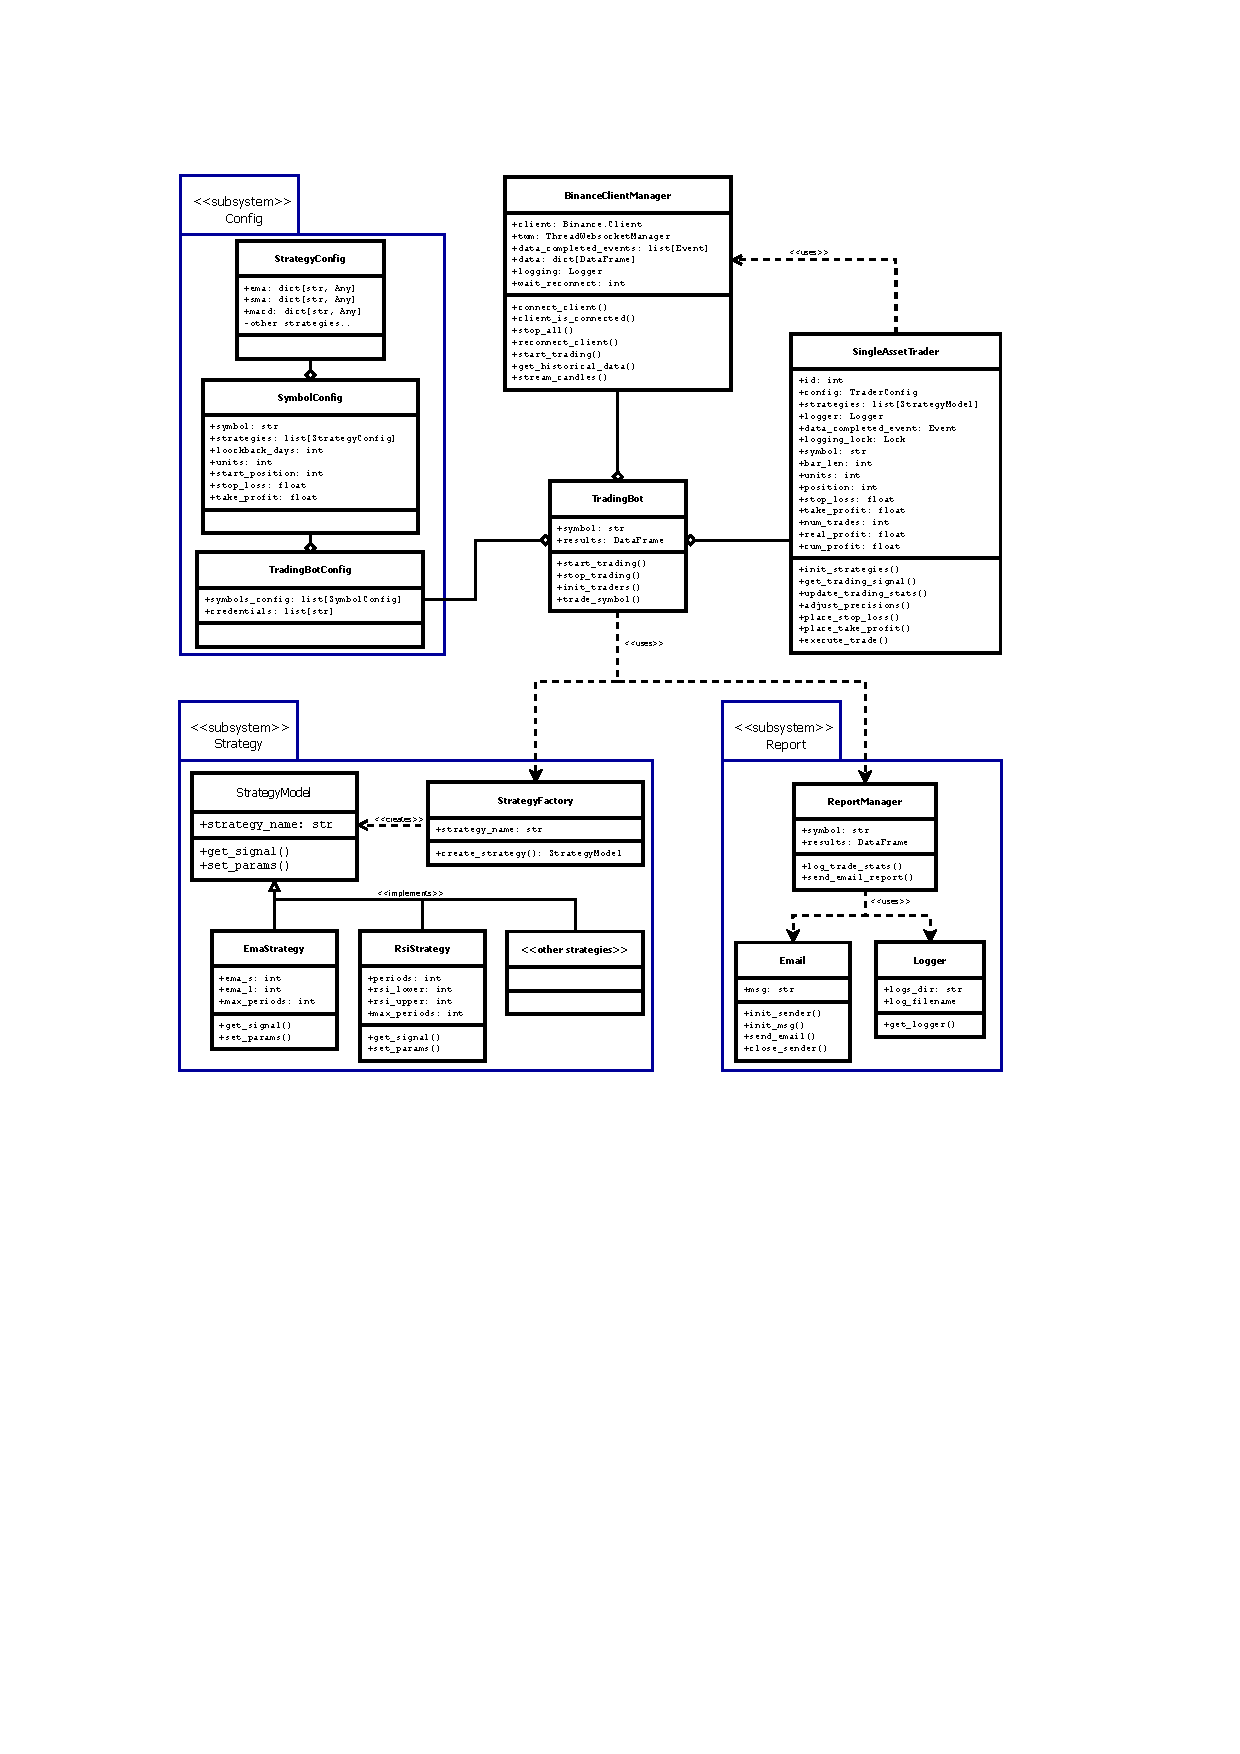
\includegraphics[page=1, trim=30mm 110mm 30mm 25mm, width=1.1\textwidth, clip]{./pdf/deployment_uml.pdf}
\caption{Architecture of the Automated Bot for Trading on the Binance Platform.}
\label{fig:deployment_arch}
\end{figure}

The deployment component of our backtesting framework is currently designed to support the Binance platform.
However, it has been architected to be extensible, allowing for potential integration with other trading platforms like Interactive Brokers for stock trading.
For any new trading platform, a dedicated client class must be provided.
In the case of Binance, all platform-specific functionalities are encapsulated within the \texttt{BinanceClientManager} class (see fig.~\ref{fig:deployment_arch}).
Any new client class should implement essential methods like \texttt{connect\_client}, \texttt{start\_trading}, \texttt{get\_historical\_data}, and \texttt{stream\_candle}.



The deployment can accommodate trading on multiple symbols using various strategies.
Since each symbol demands its specific trading details, historical data, and strategy parameters, an instance of the \texttt{SingleAssetTrader} class is created for every symbol.
This instance runs on its own dedicated thread. The \texttt{TradingManager} class ensures synchronization and coordination amongst all the components.

Configuration for trading is handled via a JSON config file.
This file specifies details like which symbols to trade on, the strategies for each symbol, their respective parameters, and more.
The \texttt{StrategyFactory} is responsible for instantiating the defined strategy models for each symbol.
These models use the retrieved historical data to generate trading signals. The \texttt{SingleAssetTrader} instances then act on these signals, placing buy or sell trades as necessary.

All trading activities are logged using a central logging system. Additionally, the framework supports email notifications for key trading events.
  % Deployment

\input{utilities.tex}  % Utilities

\input{data_retriever.tex}  % Historical Data

%
\begin{figure}[h]
\dirtree{%
.1 backtester.
.2 historical\_data.
.3 BTCUSDT
.3 ETHUSDT
.3 \ldots.
.2 \ldots.
.2 utilities.
.3 credentials.py.
.3 data\_plot\_ml.py.
.3 logger.py.
.3 performance.py.
.3 report\_email.py.
.3 data\_utils.
.4 data\_loader.py.
.4 data\_manager.py.
.4 data\_retriever.py.
.4 ml\_data\_manager.py.
.4 ml\_feature\_engineer.py.
.3 {\textbf{plot\_utils}}.
.4 {\textbf{backtesting\_plotter.py}}.
.4 {\textbf{ml\_model\_evaluator.py}}.
}

\caption{Directory structure of the project.}\label{fig:projectStructure}
\end{figure}  % Documentation (docs)
\chapter{Conclusion and Future Work}

\section{Conclusion}
This project was a big challenge, and I really learned a lot in this journey.
It made me even more excited about algorithmic trading and the application of data science for it.
I'm now eager to build better models, explore different assets and markets, and add new features into the backtesting framework as mentioned in the next section for "Future Work".
I'm more motivated than ever to push my limits, see what more I can achieve, and am very curious about the outcomes of the experiments.

\section{Further Work}
In the continued development of the backtesting framework, several enhancements and updates are planned:

\begin{itemize}
    \item Implementation of regression-based and deep learning-based backtesting strategies.
    \item Development of an assembler that leverages multiple strategies from diverse machine learning and deep learning paradigms such as regression and classification.
    \item Integration of deep reinforcement learning for advanced trading strategies.
    \item Consideration for automated portfolio management functionalities.
    \item Exploring the incorporation of Natural Language Understanding for sentiment analysis.
Potential data sources for this sentiment analysis include platforms like Twitter, Reddit, and other trading-relevant sources.
    \item Adding notifications about trades using a Telegram bot.
    \item Adding support for backtesting and trading stocks with the Interactive Brokers platform.
    \item Incorporating more optimization techniques.
    \item Configuration options for backtesting and deployment for both long-only and long-short strategies.
\end{itemize}

Adding these features will enhance the flexibility of the backtesting framework, making it more resilient, and accurate.


%\input{miscellaneous.tex}  % Miscellaneous

%\input{appendix.tex}  % Appendix

%\input{conclusion_future_enhancements.tex}  % Conclusion & Future Enhancements
    
 
%%%%%%%%%%%%%%%%%%%%%%%%%%%%%%%%%%%%%%%%%%%%%%%%%%%%%%%%%%%%%%%%%%%%%%%%%%%%%%%
\bibliographystyle{unsrt}
\bibliography{references.bib}

\end{document}
